\chapter{Techniques}
\label{techniques}

\section{Scanning Tunneling Microscopy - STM}

The main technique used in this study is scanning tunneling microscopy (STM), and more specifically the Aarhus STM. The Aarhus STM is an enhancement of the original version invented by Heinrich Rohrer and Gerhard Binnig in 1981.\cite{aarhusSTM} The STM is used to create surface images with atomic resolution of conducting samples, which makes the technique irreplaceable in this study.\\
\begin{wrapfigure}{r}{0.32\textwidth}
  \begin{center}
    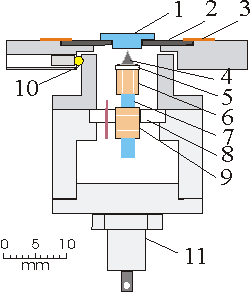
\includegraphics[width=0.32\textwidth]{aarhusSTM}
  \end{center}
  \caption{Schematic of the aarhus STM. \cite{aarhusSTM}}
  \label{aarhusSTM}
\end{wrapfigure}
Images of the sample surface are made from scanning the sample surface with a very sharp metal tip. As the sample is scanned, the tunneling current between the tip and the sample is mapped, in order to create a topographical image of the surface. The high sensitivity of the STM stems from the tunneling transmittivity which depends exponentially on the distance between the tip and the sample. The distance to the surface is measured indirectly by the tunneling current which changes by about a factor of 10 for every ångstrøm.\cite{STMbinnig} A figure of the aarhus STM is shown in figure \ref{aarhusSTM}. The sample (1) is positioned within the Tantalum sample holder (2) and both are held tight by clamps (3). The STM tip held by a macor holder (5) is seen just above the sample (4) and this is controlled by the piezo scanner tube (6). In continuation of the scanner tube, a rod (7) is mounted which extends through another configuration of piezo elements abbreviated "The inchworm". This inchworm motor, held by another macor ring (8), is able to clamp to the rod and either expand or contract, in order to approach and retire the tip from the sample. The STM is thermally isolated from the rest of the environment by quartz balls (10). If the temperature drops during cooling despite the thermal isolation,  a zener diode (11) is mounted in order to heat the STM.\\
\\
At relatively large distances the vacuum barrier that the electrons perceive is too high, and no tunneling occurs. As the distance between the sample and the tip is reduced the probability of an electron tunneling through the vacuum barrier increases until a certain point where tunneling happens. In order to achieve tunneling, the electrons need an energy at least equal to the work function given by; $\phi = E_{vac} - E_F$, where $E_{vac}$ is equal to the energy of the vacuum barrier and $E_F$ is the energy at the fermi level. To keep a current flowing a bias is applied between the sample and the tip. The energy of the fermi levels are altered by $eV$, where V is the voltage difference. This voltage difference establishes a constant flowing tunneling current, which can be calculated using the Wentzel-Kramers-Brillouin approximation. The tunneling current is given by:\cite{STMbog}
\begin{align}
  I = \int_0^{eV} \rho_s(E,r) \rho_t(E-eV,r)T(E,eV,r)dE,
  \label{eq:Iint}
\end{align}

where $\rho_s(E,r)$ and $\rho_t(E-eV,r)$ are the local densities of states (LDOS) at energy $E$ at the position r. $T(E,eV,r)$ is the tunneling transmission probability, for electrons with energy $E$ and an applied voltage of $eV$. When the applied voltage, $eV < 0$, the sample is negatively biased, and when $eV > 0$ the sample is positively biased.\\
The tunneling transmission probability is given by the following:\cite{STMbog}
\begin{align}
  T(E,eV) = \text{exp}\left( -\frac{2Z\sqrt{2m}}{\hbar} \sqrt{\frac{\phi_s + \phi_t}{2}+\frac{eV}{2}-E} \right),
  \label{eq:TTP}
\end{align}

where $Z$ is the distance between the sample and the tip, and $m$ is the mass of the electron. $\phi_s$ and $\phi_t$ are the workfunctions of the sample and the tip respectively. From this expression it is seen that once the sample is negatively biased, the limits in the integral range from 0 to $eV<0$. Equation \ref{eq:TTP} then returns the highest probability at E = 0, which is the energy at the fermi level of the sample. In contradiction, at a positive sample bias, equation \label{eq:Iint} has the limits 0 to $eV>0$. Now equation \ref{eq:TTP} returns the highest probability at the energy $E = eV$, which is the energy at the fermi level of the tip. This means the negatively biased electrode always has the highest tunneling transmission probability, and the electrons always flow from this to the positively biased electrode.\\
The tunneling current can be calculated, assuming that the density of states of the sample and the tip are constant and that $eV \ll \phi_{s,t}$.\cite{STMbog,PhysRevLett.49.57}
\begin{align}
  I = \rho_s \rho_t V \: \text{exp}\left(-\frac{2\sqrt{2(\phi_s+\phi_t)m}}{\hbar}Z \right).
  \label{eq:TC}
\end{align}

From this it is seen that the tunneling current, as mentioned, depends exponentially on the distance to the sample. Furthermore it is seen that the tunneling current depends on the applied bias, the LDOS of the sample and the tip, and their respective workfunctions.

\section{Temperature Programmed Desorption - TPD}

The desorption kinetics of hydrogen from the graphene on Ir(111) surface is studied by temperature programmed desorption (TPD). Here the temperature of the sample is raised as a function of time. The temperature program, $\beta (t) = \frac{dT}{dt}$, is commonly a linear ramp with a rate ranging from $10^{-1}$ to $10^2$ Ks$^{-1}$.\cite{TPDbog} The adsorption versus desorption rate is studied by monitoring the time evolution of the coverage of the sample denoted $\theta$. The coverage of a given adsorbate is given as the number of adsorbates on the surface as a percentage of the number of adsorbate sites. The time evolution of the coverage is naturally given by the rate of adsorption, $R_a$, subtracted by the rate of desorption, $R_d$. $R_a$ and $R_d$ is given by:\cite{TPDbog}
\begin{align}
R_a = \frac{S(\theta , T) P a_s}{\sqrt{2\pi m k_B T}} \qquad R_d = r_d(\theta, T)\theta^n
\end{align}

\begin{wrapfigure}{r}{0.32\textwidth}
  \centering
  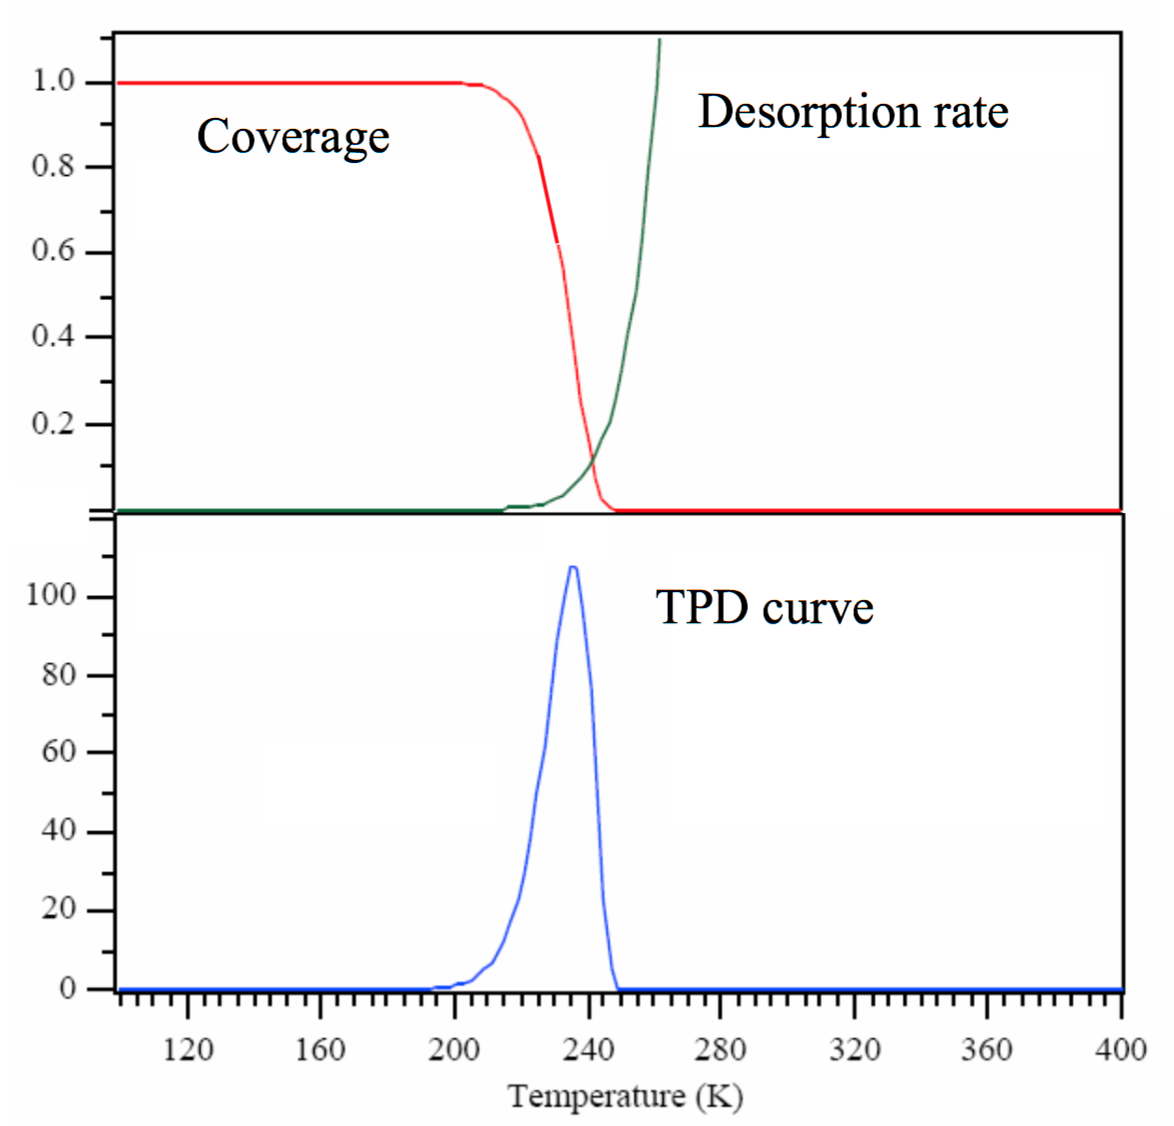
\includegraphics[width=0.32\textwidth]{TPDexample}
  \caption{Top: Surface coverage and desorption rate. Bottom: Example of TPD curve. \cite{desorpslides}}
  \label{TPDtheoryexample}
\end{wrapfigure}
For $R_a$; the initial factor $S(\Theta ,T)$ is the sticking factor, which is a substrate dependant function describing the probability of an adsorbate to stick to the surface. The second factor describes the flux of atoms impinging the surface, and this expression is known as the Hertz-Knudsen equation. $R_d$ is described as a rate of desorption multiplied by $\theta^n$, where n is the desorption order. Common desorption orders are, $n = 1$ describing molecular desorption, or $n=2$ describing associative desorption where species recombine on the surface as they desorb. During these experiments it is assumed that hydrogen adsorbed to graphene on Ir(111) has a first order desorption rate.\\
When conducting the TPD measurement the adsorbates desorb from the surface at a certain rate, until the surface is clean. The desorbed molecules are analysed by a quadropole mass analyzer. A typical evolution of the coverage and rate of desorption is seen in Figure \ref{TPDtheoryexample} as well as a typical TPD curve measured by the quadropole. Here it is seen that the rate of desorption, in theory, rise exponentially with the temperature. In practice, however, the counts of desorbed molecules eventually fall off to zero, as the surface coverage approach zero. The number of desorbed molecules can be described by the Polanyi-Wigner equation, which is given by: \cite{TPDbog, TPDekstra}
\begin{align}
  I(T) \thicksim - \frac{d\theta}{dt} = v(\theta,T)\cdot \theta^n \cdot \: \text{exp}\left(\frac{-E_{des}(\theta,T)}{k_BT}\right),
\end{align}

Where I(T) is the number of molecules and $v(\theta,T)$ abbreviated the exponential pre factor. A simple and applicable approach to TPD spectra has been proposed by Redhead from which the desorption energy can be calculated.\cite{TPDbog} It is assumed that a first order desorption from the surface is happening. Furthermore the exponential pre factor as well as the desorption energy is assumed to be coverage independent. The energy of desorption is then approximated by the following:\cite{berlinslides}

\begin{align}
E_{des} \approx RT_P \left[ \frac{v T_P}{\beta} - 3.64 \right]
\label{eq:redhead}
\end{align}

This equation is used to estimate the energy of desorption from the TPD measurements. A common exponential prefactor of $v = 10^{13} s^{-1}$ is used. This factor might, however, vary between $10^{10} s^{-1}$ to $10^{20} s^{-1}$ \cite{TPDbog}. This results in a significant error from the calculated energy of desorption of $\pm$20\%.\cite{berlinslides}

\section{Low Energy Electron Diffraction - LEED}

The first loe energy electron diffraction (LEED) experiments were carried out by Clinton Davisson and Lester Germer in 1925 at Bell Labs in New York. Here sharp interference patterns  from electron scattering from small milimeter sized nickel crystals were observed. This was only few years after De Broglie had postulated the wave nature of electrons. The wavelength of electrons is given by:\cite{held1974low}
\begin{align}
  \lambda_e = \frac{h}{m_ev} = (\frac{1.50eV}{E_{kin}})^{1/2},
\end{align}

\begin{wrapfigure}{r}{0.32\textwidth}
\centering
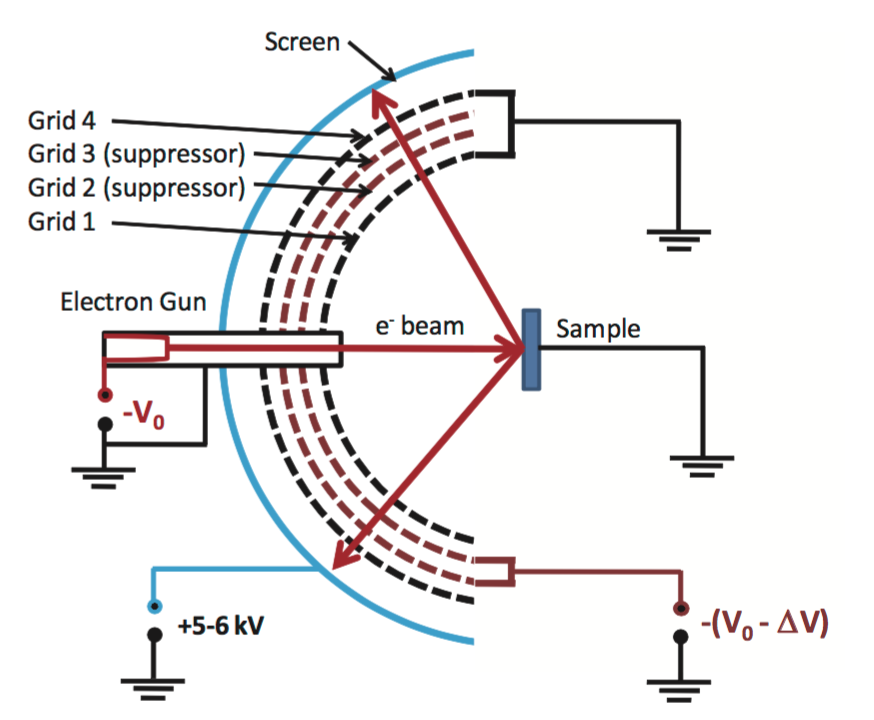
\includegraphics[width=0.32\textwidth]{LEED}
\caption{Graphical interpretaion of a LEED setup.\cite{held1974low}}
\label{leedsetup}
\end{wrapfigure}
with $m_e$ as the electron mass, and v as the velocity. Given kinetic energies ranging from few tens to few hundreds eV, the wavelength is of the order of 1Å, which is a typical interatomic distance. Using electron beams with these energies the crystal periodicity can therefore be determined by conducting LEED experiments. The technique is perfect for determining the surface geometries of samples since the inelastic mean free path of the electrons is around 1 nm.\cite{held1974low}\\
The basic principle of LEED is based on the elastic scattering of electrons. An electron beam with an energy, within the previously mentioned interval, is directed at the sample surface. Scattering of the electrons take place, and the pattern is visualised on a sensitive screen. A typical LEED setup is visualised in Figure \ref{leedsetup}. The wave vector of the diffracted electrons are given by the reciprocal lattice vectors of the sample surface:
\begin{align}
  k_{||,out} (n_1,n_2) = k_{||,in} + n_1a^*_1 + n_2a^*_2
\end{align}
This is however only component of the diffracted beam that is parallel to the incident beam. The z-component is given as:
\begin{align}
  k_{z,out}(n_1,n_2) = \left[\frac{2m_eE_{kin}}{h^2}-|k_{||,out}(n_1,n_2)|^2\right]^{1/2}
\end{align}
In order to get a diffraction spot, the square root of the right hand side must be real. This means that the number of visual diffraction spots increases with the incident beam energy.
